% !TeX spellcheck = en_US
\documentclass[a4paper,fleqn,11pt]{article}

% header
%% Packages 

% Styling TOC
\usepackage{tocloft}
\setlength\cftaftertoctitleskip{1cm}
\usepackage[nottoc]{tocbibind}

% Mathe Packages
\usepackage{amsmath,amssymb,epsfig,amsthm,amsfonts,bbm,textcomp}

% Grafiken
\usepackage[font=normalsize,aboveskip=0pt,belowskip=0pt,labelfont=bf]{caption}
\captionsetup{justification=centering,singlelinecheck=false}
\usepackage[edges]{forest}
\usepackage{tikz}
\usetikzlibrary{arrows,intersections,decorations.pathreplacing}
%\usetikzlibrary{angles,quotes}
\usepackage[utf8]{inputenc}
\usepackage[T1]{fontenc}
\usepackage{lmodern}
\usepackage[english]{babel}

% Seiten Layout
\usepackage{float} 				
\usepackage[top=3cm,bottom=3cm,left=3cm,right=3cm,a4paper]{geometry}  
\usepackage[onehalfspacing]{setspace}
\usepackage{color}
\usepackage{enumitem}

% Fussnoten
\usepackage[flushmargin,hang]{footmisc}
\usepackage{listings}
\usepackage[hyphens]{url}
\usepackage[hidelinks]{hyperref}


% Tabellen
\usepackage{longtable} 			% Lange, mehrseitige Tabelle
\usepackage{tabularx}
\usepackage{array,hhline}
\usepackage{booktabs}			% Linien zwischen Zeilen 
\usepackage{multirow}			% Verknüpfte Zellen über Zeilen hinweg
\usepackage{dcolumn}			% Erlaubt variable Orientierung am Decimalpunkt innerhalb einer Zelle
\usepackage{siunitx}

% References
\usepackage{natbib}






\begin{document}

% title page
%
% header

\pagenumbering{Roman}

\title{\huge Forecasting Swiss Exports using Bayesian \\Forecast Reconciliation}

\author[$\dagger$]{Florian Eckert}
\author[$\ddagger$]{Rob J. Hyndman}
\author[$\ddagger$]{Anastasios Panagiotelis}
\affil[$\dagger$]{\small KOF Swiss Economic Institute, ETH Zurich}
\affil[$\ddagger$]{\small Department of Econometrics and Business Statistics, Monash University}
\date{July 2019}

\maketitle
\begin{abstract}
\noindent This paper conducts an extensive forecasting study on 13,118 time series measuring Swiss goods exports, grouped hierarchically by export destination and product category.  We apply existing state of the art methods in forecast reconciliation and introduce a novel Bayesian reconciliation framework. This approach allows for explicit estimation of reconciliation biases, leading to several innovations: Prior judgment can be used to assign weights to specific forecasts and the occurrence of negative reconciled forecasts can be ruled out. Overall we find strong evidence that in addition to producing coherent forecasts, reconciliation also leads to improvements in forecast accuracy.

\noindent \textbf{JEL Classification:} C32, C53, E17\\
\noindent \textbf{Keywords}: Hierarchical Forecasting, Bayesian Forecast Reconciliation, Swiss Exports, Optimal Forecast Combination.
\end{abstract}
\clearpage




% table of contents
%\tableofcontents

%\clearpage

%\listoffigures
%\listoftables

%\clearpage

\pagenumbering{arabic}

			




% 2. Model	
\section{Introduction}
\label{sec:model}
Data in business analytics and economics often occurs naturally in additive hierarchical structures. For instance, sales of a car dealership can be disaggregated by brands and then further by car model of each brand. In most cases, the series at the bottom of a hierarchy can be added up in more than one unique hierarchical way to the main aggregate. This is referred to as a grouped time series by \cite{Hyndman2016}. Retail sales for example can be added up by product type or by store location. Employment data can be aggregated by age group, gender, profession or location. Figure \ref{fig:tree} gives an example of a simple grouped hierarchy with $k = 3$ levels, $m = 9$ series in total and $q = 4$ series at the bottom.
\begin{figure}[H]
	\centering
	\begin{forest}
		before packing={
			forked edges,
		}
		[{$Y_0$}
		[{$Y_{A}$}
		[{$Y_{A1}$}]
		[{$Y_{A2}$}]
		]
		[{$Y_{B}$}
		[{$Y_{B1}$}]
		[{$Y_{B2}$}]
		]
		]
	\end{forest}\hspace{1cm}
	\begin{forest}
		before packing={
			forked edges,
		}
		[{$Y_0$}
		[{$Y_{1}$}
		[{$Y_{A1}$}]
		[{$Y_{B1}$}]
		]
		[{$Y_{2}$}
		[{$Y_{A2}$}]
		[{$Y_{B2}$}]
		]
		]
	\end{forest}
	\vspace{0.4cm}
	\caption{Simple Example of a Grouped Hierarchy}
	\label{fig:tree}
\end{figure}
All hierarchies are subject to strict aggregation constraints. In order to express the constraints in this example hierarchy, $Y_t$ is defined to be a vector containing the top-down stacked observations from all levels. $Y_{k,t}$ contains the observations at the bottom level $k$ of the hierarchy and $S$ is a corresponding aggregation matrix.
\begin{align*}
\underset{(m\times 1)}{Y_t} = \begin{bmatrix}
\ Y_0\ \ \\
\ Y_A\ \ \\
\ Y_B\ \ \\
\ Y_1\ \ \\
\ Y_2\ \ \\
\ Y_{A1}\ \ \\
\ Y_{A2}\ \ \\
\ Y_{B1}\ \ \\
\ Y_{B2}\ \ 
\end{bmatrix} \quad \underset{(m\times q)}{S} &=
\begin{bmatrix}
\ 1 & 1 & 1 & 1 \ \ \\
\ 1 & 1 & 0 & 0 \ \ \\
\ 0 & 0  & 1 & 1\ \ \\
\ 1 & 0 & 1 & 0 \ \ \\
\ 0 & 1 & 0 & 1\ \ \\
\ 1 & 0 & 0 & 0 \ \ \\
\ 0 & 1 & 0 & 0 \ \ \\
\ 0 & 0 & 1 & 0 \ \ \\
\ 0 & 0 & 0 & 1\ \ 
\end{bmatrix} \quad \underset{(q\times 1)}{Y_{k,t}} = \begin{bmatrix}
	\ Y_{A1}\ \ \\
	\ Y_{A2}\ \ \\
	\ Y_{B1}\ \ \\
	\ Y_{B2}\ \ 
\end{bmatrix} 
\end{align*}
For realized data, it must hold at each point in time that $Y_t = S Y_{k,t}$. Forecasts of the individual series however usually do not fulfill these aggregation constraints. Incoherences may arise due to model bias, varying information sets or different models used when predicting the individual series in a hierarchy. Following \cite{Gross1990}, a simple way to ensure consistency is the «bottom-up» approach. This means that only the bottom level series are forecasted and then added up according to the hierarchical structure. It implies that forecasts from higher levels are not taken into account, even though they are usually better to predict than the noisier series at the bottom of a hierarchy. Another possibility is the «top-down» approach described in \cite{Athanasopoulos2009}, where the forecast of the top level series is disaggregated according to the historical or forecasted proportions at lower levels. This approach relies on the characteristics of the top series and does not take into account the predictions at lower levels. A compromise is given by the «middle-out» approach, where the forecasts at an intermediate level of the hierarchy are summed up to get the higher levels and disaggregated to obtain lower level predictions.

Many empirical studies have shown that forecast combinations improve accuracy because of information pooling and the averaging over misspecification biases and measurement errors.\footnote{See for instance \cite{Timmermann2006} or \cite{Watson2004} for a comprehensive overview.} Similarly, it is beneficial to combine information from all forecasts in a hierarchy. \cite{Hyndman2011} have shown that optimal, reconciled predictions can be obtained using the following regression approach.
\begin{align}
Y_t(h) &= S\beta_{h} + e_t(h)
\end{align}
where $Y_t(h)$ is an ($m \times 1$) vector containing the h-periods-ahead forecasts at time $t$ for each level in the hierarchy. $\beta_{h}$ represents the optimal predictions at the bottom level that minimize the deviations between the base forecasts and the consistent hierarchy. The reconciliation error term $e_t(h)$ follows a normal distribution with mean zero and covariance matrix $\Sigma_h$. There is obviously a high level of heteroskedasticity in the error terms, which is why the simple ordinary least squares regression approach often leads to poor results. In order to account for this, $\beta_h$ can be estimated from a weighted least squares regression.
\begin{align}
\label{eq:reg}
\beta_{h} &= \left(S'W_h^{-1}S \right)^{-1} S'W_h^{-1}Y_t(h)
\end{align}
Intuitively, $\beta_h$ minimizes the reconciliation error, which is the distance between actual and reconciled forecasts across the entire hierarchy. \cite{Hyndman2016} use the covariance matrix $\Sigma_h$ of the $h$-step-ahead base forecast errors as the weighting matrix $W_h$. This «GLS» approach decreases the weight of forecasts with a high prediction error in the regression. In the «MinT» approach, \cite{Wickramasuriya2015} use the covariance matrix of the $h$-step-ahead reconciled forecast errors, which they show results in the best linear unbiased reconciled forecasts. Lastly, the «nseries» approach, proposed by \cite{Athanasopoulos2017}, uses weights based on the number of series aggregated at each node.\\

This paper contributes to the literature on optimal hierarchical forecasting by constructing a Bayesian reconciliation framework. It introduces an explicit definition of the coherency errors as model parameters in section \ref{sec:model}. Probabilistic reconciliation takes the uncertainty surrounding these parameters into account and leads to reconciled density forecasts. Furthermore, flexible shrinkage priors enable the model to shrink selected reconciled forecasts towards their base forecast. In section \ref{sec:appl}, the method is compared with existing optimal and basic reconciliation techniques using a comprehensive hierarchical dataset of Swiss goods exports, grouped geographically and categorically.

\clearpage

\section{Bayesian Forecast Reconciliation}
\label{sec:model}
\subsection{Model}
Density forecasts have the benefit of providing additional information about the uncertainty surrounding a measure of central tendency. Recent years have seen an increase in the use of model combinations for density forecasts, such as \cite{Kapetanios2015} and \cite{Cesur2016}. In their spirit, the predictive densities of the $m$ base forecast models are approximated by drawing $n$ samples from the respective distributions. There are $n$ vectors $\hat{y}_{i}$ of length $m$ that contain a draw $i$ from each predictive distribution.\footnote{Since every forecast horizon is reconciled independently, the time subscripts are dropped from now on to simplify notation.} The error term consists of two components, a prediction error $e_{i}$ and a reconciliation error $\alpha$. The latter can be interpreted as a fixed effect that is unique to each forecasted variable. In other terms, $\alpha$ is the difference between the unreconciled forecast mean $\hat{y}$ and the reconciled forecast mean $\tilde{y}$. The interpretation of $\beta$ depends on the definition of $S$, but in general it estimates the mean of the bottom level reconciled forecasts. The following equation can then be used to model the forecast reconciliation.
\begin{align}
\label{eq:main}
\begin{tabular}{ccccccccc}
	$\hat{y}_i$ & $=$ & $\alpha$ & + &$S$ & $\times$ & $\beta$ & $+$ & $e_i$ \\
	$\scriptscriptstyle (m\times 1)$ & & $\scriptscriptstyle (m\times 1)$  & & $ \scriptscriptstyle (m\times q) $ & & $\scriptscriptstyle (q\times 1)$ & & $\scriptscriptstyle (m\times 1)$
\end{tabular}
\end{align}
where $e$ follows a normal distribution with mean zero and covariance matrix $\Sigma$. While $\Sigma$ is not singular by definition because the forecasts in $\hat{y}_{i}$ are not reconciled, it might be near-singular if the base forecasting models are estimated jointly. In the much more common case of independently estimated univariate models, $\Sigma$ is simply a diagonal matrix. It is however possible to order the draws from each predictive distribution before stacking them into $\hat{y}_{1},\hdots,\hat{y}_{n}$, which artificially introduces correlation into $\Sigma$. Irrespective of this, the unreconciled forecasts $\hat{y}_{i}$ follow a multivariate normal distribution.
\begin{align}
\hat{y}\ |\ \alpha,\beta,\Sigma \sim N(\alpha + S\beta,\Sigma)
\end{align}
We are however interested in the reconciled forecasts $\tilde{y} \sim N(S\beta,\Sigma)$, which can be obtained by conditioning on $\alpha = 0$. An estimate for the reconciled means is therefore given by the conditional expectation function.
\begin{align}
	E(\tilde{y}) = E(\hat{y}|\alpha = 0,\beta,\Sigma) = \int \hat{y} f_{\hat{y}|\alpha,\beta,\Sigma}(0,\beta,\Sigma) d\hat{y} 
\end{align}
The reconciled conditional distribution and the corresponding moments can be retrieved from the Gibbs sampling algorithm described in the following subsection.\\

\clearpage

\subsection{Estimation}
To account for cross-equation correlations, the reconciliation problem in (\ref{eq:main}) can be expressed as a system of seemingly unrelated regressions. Since the explanatory variables are the same for each equation, it is a special case of the SUR model in \cite{Zellner1962}. However, the parameters are impossible to estimate directly because of perfect multicollinearity in the regressors $I_m$ and $S$. This represents an ill-posed problem because there is no unique solution. A convenient answer to this identification problem is given by Bayesian regularization methods. Following \cite{Farebrother1978}, the regression is partitioned in order to separate the parameters that cause multicollinearity. By imposing prior shrinkage on the reconciliation errors $\alpha$, it will be possible to find a unique solution to the entire estimation problem.
\begin{align}
	\sum_{i=1}^n \hat{y_i} &= \sum_{i=1}^n \left(I\alpha + S\beta + e_i\right),\quad e_i \sim N(0,\Sigma)
\end{align}
In Bayesian statistics, data is considered to be fixed and parameters are treated as random variables. The researcher has a prior belief about the distribution of the parameters in a model. After observing the data, this prior belief is combined with the likelihood according to Bayes' theorem in order to obtain the posterior distribution of the parameters. This principle can be applied to $\alpha$, $\beta$ and $\Sigma$ in the reconciliation regression.
\begin{align}
	f(\alpha, \beta, \Sigma\ |\ \hat{y}) \propto f(\hat{y}\ |\ \alpha, \beta, \Sigma) \times f(\alpha, \beta, \Sigma)
\end{align}
In other words, the posterior distribution of the bottom-level forecasts is proportional to the likelihood of the hierarchy to be consistent times the prior distribution of the parameters. In order to approximate the distribution of $\hat{y}$, we draw $n$ $h$-periods-ahead-predictions $\hat{y}_i$ from their unreconciled predictive distributions. The likelihood function for the data is then given by 
\begin{align*}
f(\hat{y}\ |\ \alpha,\beta,\Sigma) \propto \frac{1}{|\Sigma|}\exp\left[\frac{1}{2} \sum_i (\hat{y}_i - \alpha - S\beta)'\Sigma^{-1}(\hat{y}_i - \alpha - S\beta)\right]
\end{align*}
and the posterior distribution is accordingly
\begin{align*}
f(\alpha,\beta,\Sigma\ |\ \hat{y}) & \propto \frac{1}{|\Sigma|^{n/2}}\exp\left[-\frac{1}{2} \sum_i (\hat{y}_i - \alpha - S\beta)'\Sigma^{-1}(\hat{y}_i - \alpha - S\beta)\right] \\
&\times \exp \left[-\frac{1}{2}(\alpha - a_0)'A_0^{-1}(\alpha - a_0)\right] \\
&\times \exp \left[-\frac{1}{2}(\beta - b_0)'B_0^{-1}(\beta - b_0)\right] \\
&\times \frac{1}{|\Sigma|(v_0 - m - 1)} \exp \left[-\frac{1}{2} tr(R_0^{-1}\Sigma^{-1}) \right]
\end{align*}
Following \cite{Percy1992}, we get the marginal distributions of $\alpha$, $\beta$ and $\Sigma$ by approximating the joint posterior distribution via Gibbs sampling from the conditional distributions. After choosing a set of arbitrary starting values, the following steps are repeated until convergence.

\begin{enumerate}
\item \textbf{Draw $\beta$ conditional on $\alpha,\Sigma,\hat{y},S$}\\
The parameter $\beta$ is the mean of the bottom level forecasts, given an appropriate aggregation matrix $S$. The conditional posterior distribution is given by
\begin{align}
\beta\ |\ \alpha,\Sigma,\hat{y} &\sim N(b_1,B_1)
\end{align}
where
\begin{align*}
B_1 &= \left(\sum_i S'\Sigma^{-1}S + B_0^{-1}\right)^{-1} \\
b_1 &= B_1 \left(\sum_i S'\Sigma^{-1} (\hat{y}_i - \alpha) + B_0^{-1}b_0\right)
\end{align*}
Unless there is reason to believe otherwise, the priors $b_0$ and $B_0$ should be chosen as uninformative as possible. In some cases, negative values in the reconciled forecasts are a concern. This issue can be resolved quite uncomplicated during the sampling process by discarding draws of $\beta$ that contain negative entries.\\

\item \textbf{Draw $\Sigma$ conditional on $\alpha,\beta,\hat{y},S$}\\
$\Sigma$ is the covariance matrix of the prediction errors. Depending on how the draws from each predictive distribution are ordered in $Y$, there is more or less structure in the off-diagonal elements. $\Sigma$ can be drawn from an inverse Wishart distribution.
\begin{align}
\Sigma\ |\ \alpha,\beta,\hat{y} \sim W^{-1}(v_1,R_1)
\end{align}
where
\begin{align*}
v_1 &= v_0 + n\\
R_1 &=  \left( R_0^{-1} + \sum_i (\hat{y}_i - \alpha - S \beta)'(\hat{y}_i - \alpha - S \beta) \right)^{-1}
\end{align*}
It is useful to set an almost uninformative prior with $v_0$ and $R_0$ very close to zero, which introduces a tiny bit of noise into the reconciled forecasts. This has negligible impact on the posterior distribution, but ensures that $\Sigma$ is nonsingular in the case where a base forecast has no variation. If there is no correlation between the base forecast distributions, for instance if they originate from independent univariate models, it might be faster for large hierarchies to draw the variances equation-by-equation from an inverse gamma distribution.\\

\item \textbf{Draw $\alpha$ conditional on $\beta,\Sigma,\hat{y},S$}\\
It is necessary to impose an informative prior on the reconciliation errors $\alpha$ in order to achieve identification. This process of adding information to solve an ill-posed problem is referred to as regularization\footnote{Parameter shrinkage  has been studied extensively in the literature on regularization techniques for high-dimensional data, where penalties lead to the selection of models with fewer predictors and less variance. See for instance \cite{Polson2010} for an overview. A closely related technique to overcome multicollinearity is the adaptive ridge estimator developed by \cite{Brown1980} and extended to the seemingly unrelated regression framework by \cite{Haitovsky1987} and \cite{Firinguetti1997}.}. Furthermore, an informative prior on $\alpha$ reflects knowledge or preferences about the reconciliation errors. The prior mean $a_0$ is a vector of zeros. This assumes that the base forecasts are unbiased and therefore do not deviate systematically from the reconciled forecasts. The prior covariance matrix $A_0$ determines how strongly the reconciliation errors are allowed to deviate from zero. Setting the diagonal entries very high leads to a diffuse prior. This implies that there is no prior knowledge about the reconciliation errors and as a result, the model parameters cannot be uniquely identified. Setting the diagonal entries very close to zero leads to a strong prior. This implies that the reconciliation errors are distributed tightly around zero. In this case, the prior information dominates the informational content of the data and $\beta$ reduces to the generalized least squares estimate in \cite{Hyndman2016}. There exists an optimal solution, which can be obtained by taking into account the dependency of $\alpha$ on $\beta$ in the partitioned regression model. Equation (\ref{eq:prior1}) shows the basic reconciliation identity.
\begin{align}
	\label{eq:prior1}
	a &= \frac{1}{n}\sum_i \hat{y}_i - Sb
\end{align}
In order to eliminate $b$ from equation (\ref{eq:prior1}), both sides of the equation are multiplied by the projection matrix $S(S'W^{-1}S)^{-1}S'W^{-1}$. The resulting term is then subtracted from equation (\ref{eq:prior1}), which leaves the reconciliation errors as a function of the data and the summation matrix $S$.
\begin{align}
	\label{eq:prior2}
	(I_m - S(S'W^{-1}S)^{-1}S'W^{-1})\ a &= (I_m - S(S'W^{-1}S)^{-1}S'W^{-1})\ \frac{1}{n}\sum_i \hat{y}_i  
\end{align}
It is useful to define the idempotent residual maker $I_m - S(S'W^{-1}S)^{-1}S'W^{-1}$ as $M$. Using $\Sigma$ as the weighting matrix $W$, the residual maker generates the generalized least squares residuals that result from a regression of the reconciliation errors on the reconciled hierarchy. Because the resulting residuals are by definition the reconciliation errors, it is possible to set $Ma = a$. This simplifies equation (\ref{eq:prior2}) and disposes of the need to invert $M$.
\begin{align}
	a &= \frac{1}{n}\sum_i M\hat{y}_i 
\end{align}
Having enforced mean zero of the reconciliation errors, the prior variance $A_0$ can be chosen very diffuse. The conditional posterior distribution for $\alpha$ is therefore given by
\begin{align}
	\label{eq:alpha}
	\alpha\ |\ \beta,\Sigma,\hat{y} &\sim N(a_1,A_1)
\end{align}
where
\begin{align*}
	A_1 &= M (\Sigma/n) M' + A_0^{-1} \\
	a_1 &= \frac{1}{n}\sum_i M\hat{y}_i  + A_0^{-1}a_0
\end{align*}
The precision of this approach can be checked easily by comparing the estimate of $\alpha$ and the reconciliation errors from the fitted values. \\

Even though it is intuitive to weigh the reconciliation errors based on the predictive accuracy of the corresponding base forecast, the weighting matrix $W$ in the residual maker does not necessarily have to correspond to $\Sigma$. A low value results in a lower reconciliation error. There may exist prior information on the reliability of certain models or the requirement to fix some forecasts at specific values. This could be due to better data availability, higher suitability of a particular model or subjective judgment of the forecaster. In this case, it is of interest to selectively shrink some reconciliation errors towards zero. At the same time, it is necessary to increase the variation of the remaining elements in $\alpha$ such that they are able to capture the increased reconciliation errors at their level of the hierarchy. This can be achieved by keeping constant the total dispersion of a multivariate normal distribution. A common measure is the generalized variance described in \cite{Mustonen1997} and defined as the determinant of a covariance matrix. Using a diagonal scaling matrix $\lambda$, it is therefore possible to construct any weighting matrix $W =  \lambda\Sigma\lambda'$ as long as the product of the diagonal elements in $\lambda$ remain constant at 1. This in turn ensures that the total dispersion of the weighting matrix $W$ remains the same as the total dispersion of $\Sigma$. An example of how to shrink selected reconciliation errors is given by equation (\ref{eq:scale}).
\begin{align}
	\label{eq:scale}
	|\lambda| &= \lambda_1 \lambda_2 \hdots \lambda_m
	= \prod_{s^- = 1}^{x} \lambda_{s^-}\ \eta^{-\frac{1}{x}}   \prod_{s^+ = x+1}^{m} \lambda_{s^+}\ \eta^{\frac{1}{m-x}} = 1
\end{align}
The $x$ local variance components $\lambda_{s^-}$ are scaled down by a factor $\eta^{\frac{1}{x}}$ and the remaining $(m-x)$ components $\lambda_{s^+}$ are correspondingly scaled up by a factor $\eta^{\frac{1}{m-x}}$. The generalized variance remains at unity irrespective of the scaling factor $\eta$ and the number of series to be scaled down $x$. Other possible approaches include the weighting of each reconciliation error by the level in the hierarchy or by to the number of series at each node in the hierarchy. This allows for the replication of the «bottom-up», «middle-out» and «top-down» results.

\end{enumerate}

\noindent The Bayesian approach has the advantage that uncertainty surrounding the parameters $\alpha$, $\beta$ and $\Sigma$ is taken into account when calculating the conditional expectation of $\tilde{y}$. Convergence of the Gibbs sampler happens usually within the first hundred draws, irrespective of the starting values. It can checked by testing for stability in the recursive means of the Markov chains. After convergence is achieved, a sufficiently large sample of draws from the joint posterior is saved and evaluated.\\

\clearpage


\section{Empirical Application}
\label{sec:appl}
\subsection{Data}
We use a comprehensive dataset of Swiss foreign trade in goods. For both exports and imports, it contains the nominal value in Swiss francs of goods traded with 245 countries and dependent territories. The goods are categorized according to the economic sector, following a national nomenclature covering 14 main groups and 272 subgroups. The hierarchy is unbalanced, meaning that certain goods categories are available more disaggregated than others. This results in a hierarchy with up to 5 levels. Because of the geographical and the categorical dimension, there is no unique hierarchical structure. Following \cite{Hyndman2016}, these time series can therefore be thought of as a grouped time series. There are 63'516 time series with non-zero entries in total, 35'602 for the export hierarchy and 27'914 for the import hierarchy. The time series are available in monthly frequency from 1989 on and are not adjusted for working days or seasonality. The data is collected by the Swiss Federal Customs Administration\footnote{\url{https://www.ezv.admin.ch/ezv/en/home/topics/swiss-foreign-trade-statistics.html}} and made available in a machine-friendly data format only on basis of a subscription.\\
\begin{figure}[H]
	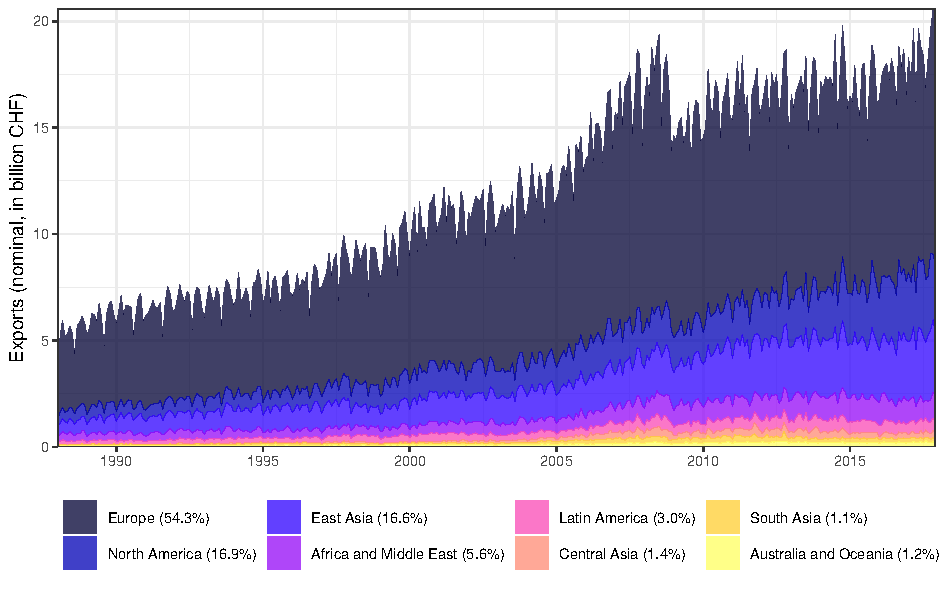
\includegraphics[width=\textwidth]{fig/fig_area_reg}
	\caption{Swiss Exports in Goods by Region}
	\footnotesize{Period from 1988-2017 in monthly frequency. Average export shares during 2017 in parentheses. Precious metals, precious and semi-precious stones, works of art and antiques are omitted due to their volatility.}
\end{figure}

\begin{figure}[H]
	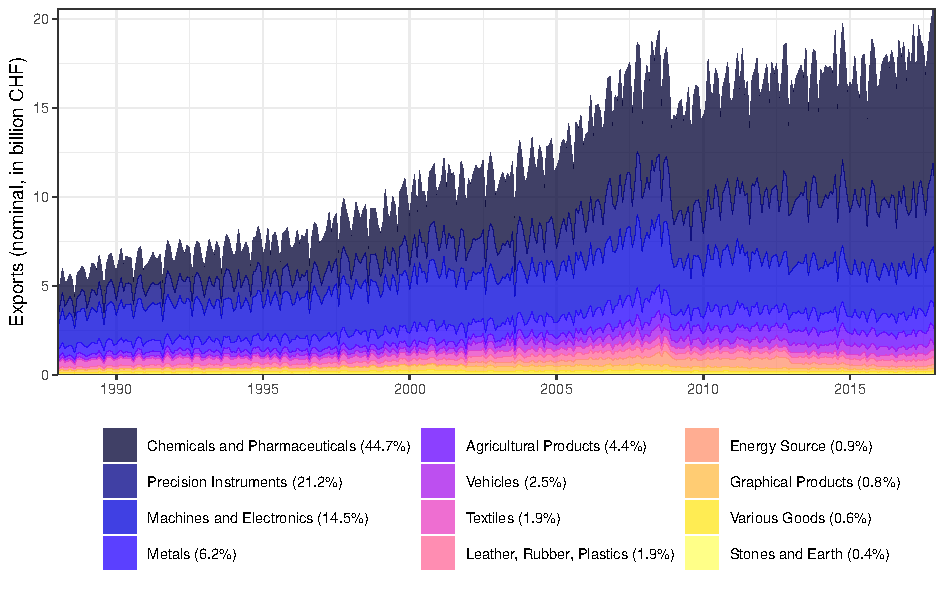
\includegraphics[width=\textwidth]{fig/fig_area_cat}
	\caption{Swiss Exports in Goods by Category}
	\footnotesize{Period from 1988-2017 in monthly frequency. Average export shares during 2017 in parentheses. Precious metals, precious and semi-precious stones, works of art and antiques are omitted due to their volatility.}
\end{figure}

 The 14 main groups are the following:
\begin{enumerate}[itemsep=-1ex,partopsep=1ex,parsep=1ex]
    \item Forestry and agricultural products, fisheries
    \item Energy source
    \item Textiles, clothing, shoes
    \item Paper, stationery and graphical products
    \item Leather, rubber, plastics 
    \item Products of the chemical and pharmaceutical industry
    \item Stones and earth
    \item Metals
    \item Machines, appliances, electronics
    \item Vehicles
    \item Precision instruments, clocks and watches and jewellery  
    \item Various goods such as music instruments, home furnishings, toys, sports equipment
    \item Precious metals, precious and semi-precious stones
    \item Works of art and antiques
\end{enumerate}

Series at the top level tend to be more predictable than those at the bottom.

\begin{figure}[H]
	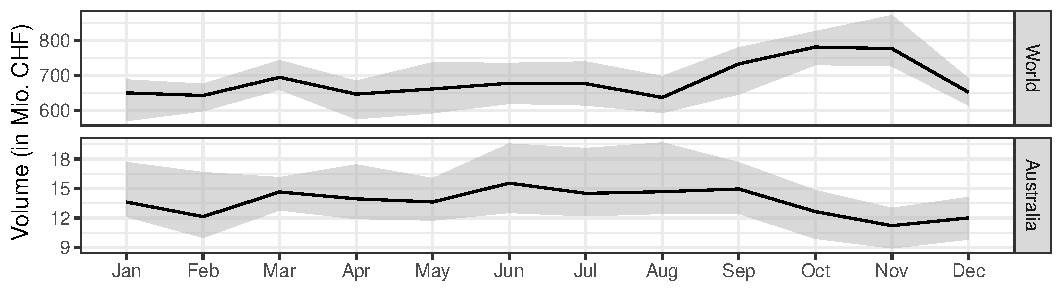
\includegraphics[width=\textwidth]{fig/fig_season}
	\caption{Exports of Food, Beverages and Tobacco to the World and Australia}
	\footnotesize{Plot demonstrates different seasonalities at different levels in a hierarchy. Line indicates average of 2012 - 2017, bands indicate minimum and maximum.}
\end{figure}

\begin{figure}[H]
	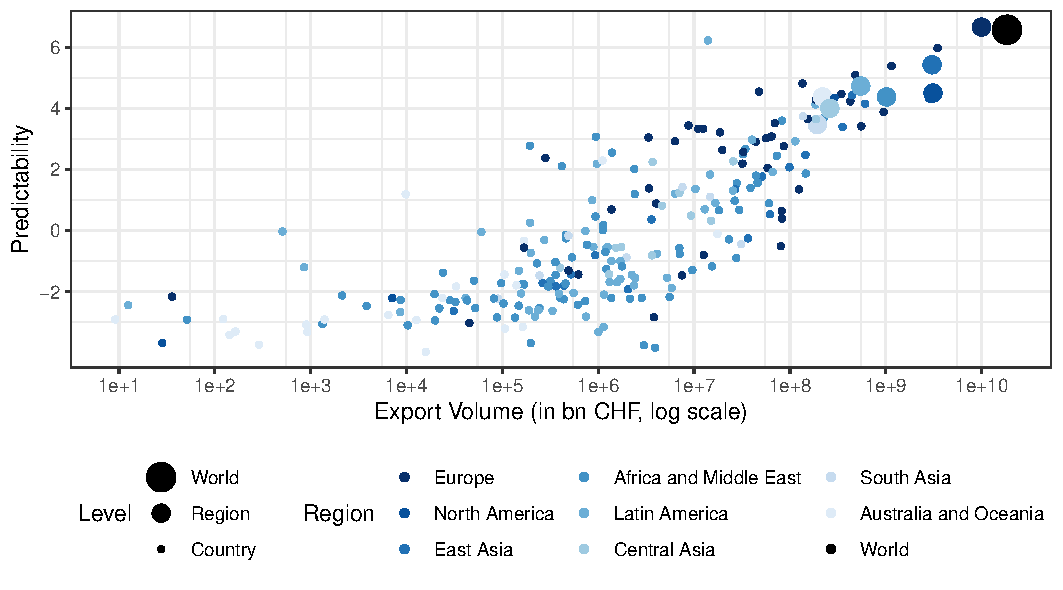
\includegraphics[width=\textwidth]{fig/fig_confetti}
	\caption{Predictability of Different Levels in a Hierarchy}
	\footnotesize{Predictability given by the first component of time series features such as trend, strength of seasonality, spectral entropy, autocorrelation.}
\end{figure}


\subsection{Results}
 Part 1: Obvious results 
 
 Part 2: Is it beneficial to use hierarchies instead of unreconciled forecasts? Which reconciliation procedures produce the best forecasts?
 \begin{figure}[H]
 	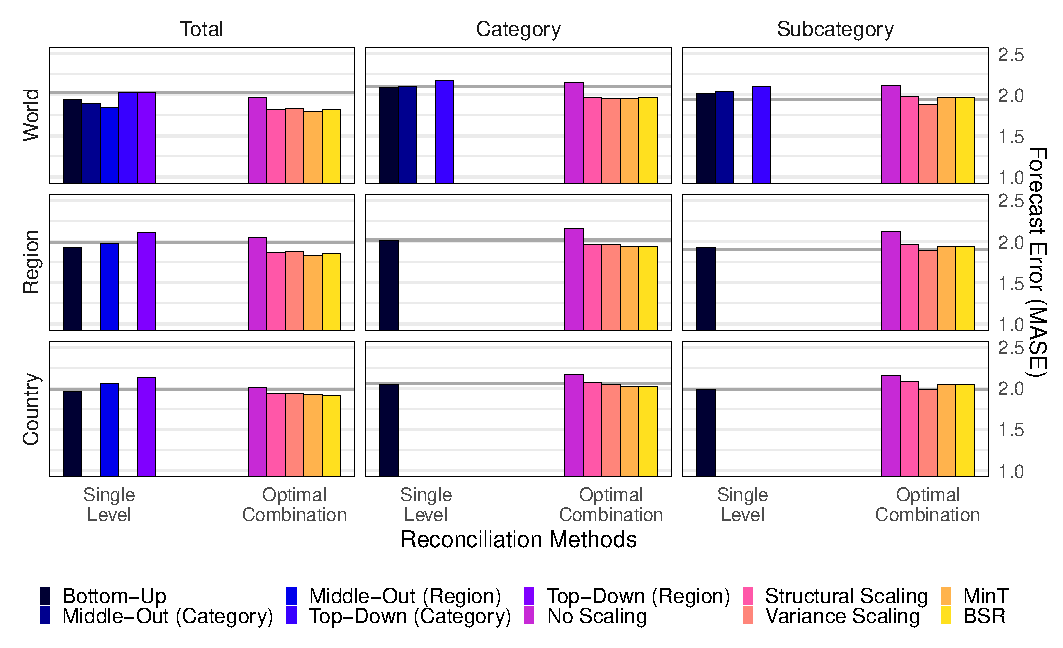
\includegraphics[width=\textwidth]{fig/fig_eval_mase}
 	\caption{Accuracy of Reconciliation Methods at Different Levels}
 	\footnotesize{Average of all time periods, forecasting horizons and methods. Lower level forecast errors are weighted by their respective export share.}
 \end{figure}

 \begin{figure}[H]
	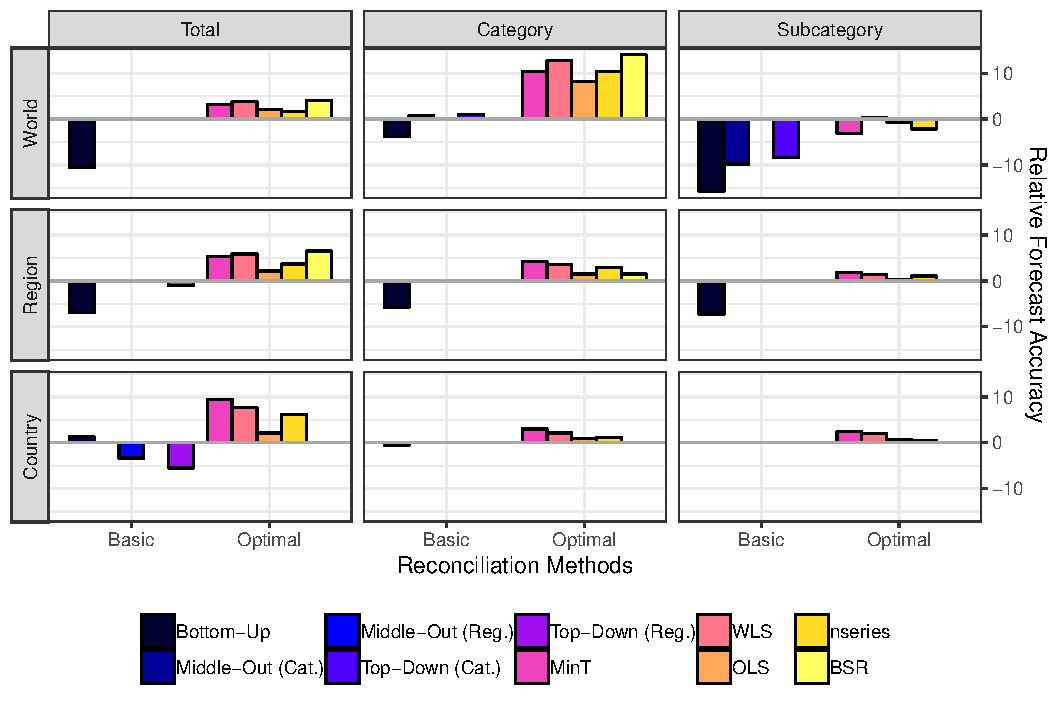
\includegraphics[width=\textwidth]{fig/fig_eval_rmse_relative}
	\caption{Accuracy of Reconciliation Methods at Different Levels}
	\footnotesize{Average of all time periods, forecasting horizons and methods. Lower level forecast errors are weighted by their respective export share.}
\end{figure}

 \begin{figure}[H]
	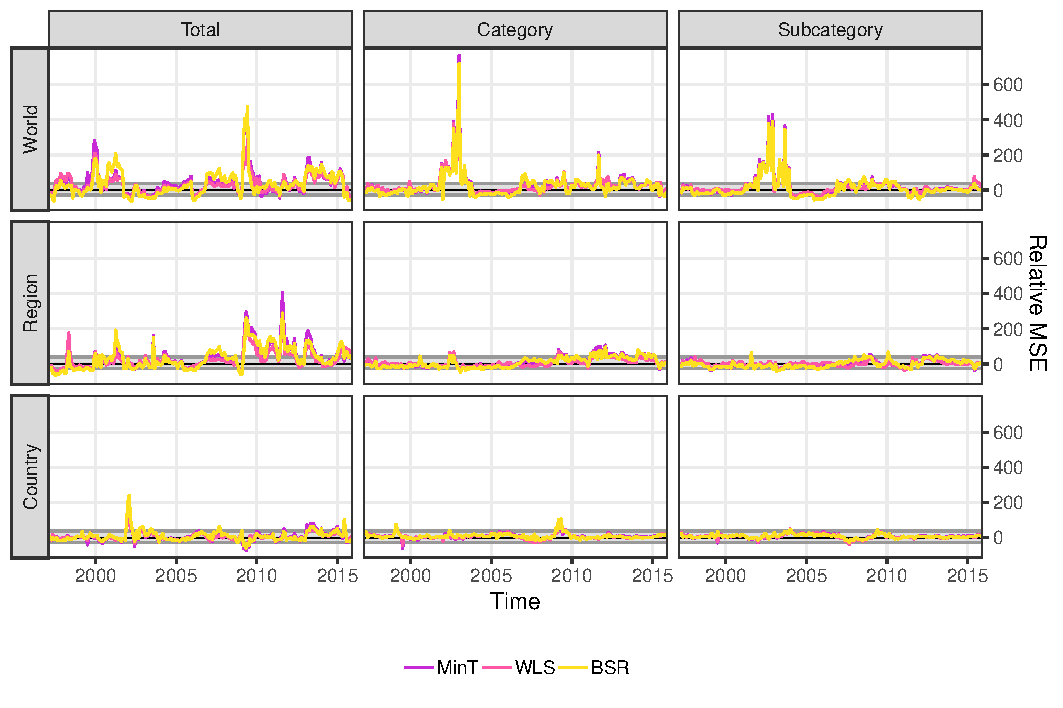
\includegraphics[width=\textwidth]{fig/fig_eval_rmse_time}
	\caption{Accuracy of Reconciliation Methods at Different Levels}
	\footnotesize{Average of all time periods, forecasting horizons and methods. Lower level forecast errors are weighted by their respective export share.}
\end{figure}
 
Part 3: How are different subcategories affected by the reconciliation? (Correlation between share of the series and improvement of forecasts)


%
%Results from running hts on the data, using the average across the root mean squared errors and mean absolute percentage errors of all series.\\
%\begin{table}[H]
%\centering
%\caption{Forecast Accuracy by Standard Aggregation Methods}
%\small
%\begin{tabularx}{\textwidth}{Xcclcclcclcc}
%\toprule
%& \multicolumn{2}{c}{Overall} & & \multicolumn{2}{c}{2003-2007} & & \multicolumn{2}{c}{2008-2012} & & \multicolumn{2}{c}{2013-2018}\\
%\cmidrule{2-3} \cmidrule{5-6} \cmidrule{8-9} \cmidrule{11-12}
%& \scriptsize{MAPE} & \scriptsize{RMSE} & & \scriptsize{MAPE} & \scriptsize{RMSE} & & \scriptsize{MAPE} & \scriptsize{RMSE} & & \scriptsize{MAPE} & \scriptsize{RMSE}\\ 
%\midrule
%Bottom-up &  &  &&  & && & && & \\ 
%\quad \scriptsize{ETS} & 2.3 & 2.3  && 2.3 & 2.3 && 2.3 & 2.3 && 2.3 & 2.3\\ 
%\quad \scriptsize{ARIMA} & 2.3 & 2.3  && 2.3 & 2.3 && 2.3 & 2.3 && 2.3 & 2.3\\
%\addlinespace
%Middle-out &  &  &&  & && & && & \\ 
%\quad \scriptsize{ETS} & 2.3 & 2.3  && 2.3 & 2.3 && 2.3 & 2.3 && 2.3 & 2.3\\ 
%\quad \scriptsize{ARIMA} & 2.3 & 2.3  && 2.3 & 2.3 && 2.3 & 2.3 && 2.3 & 2.3\\
%\addlinespace
%\multicolumn{3}{l}{Top-down (Gross-Sohl A)} &&  & && & && & \\ 
%\quad \scriptsize{ETS} & 2.3 & 2.3  && 2.3 & 2.3 && 2.3 & 2.3 && 2.3 & 2.3\\ 
%\quad \scriptsize{ARIMA} & 2.3 & 2.3  && 2.3 & 2.3 && 2.3 & 2.3 && 2.3 & 2.3\\
%\addlinespace
%\multicolumn{3}{l}{Top-down (Gross-Sohl F)} &&  & && & && & \\ 
%\quad \scriptsize{ETS} & 2.3 & 2.3  && 2.3 & 2.3 && 2.3 & 2.3 && 2.3 & 2.3\\ 
%\quad \scriptsize{ARIMA} & 2.3 & 2.3  && 2.3 & 2.3 && 2.3 & 2.3 && 2.3 & 2.3\\
%\addlinespace
%\multicolumn{3}{l}{Top-down (Forecast Proportions)} &&  & && & && & \\ 
%\quad \scriptsize{ETS} & 2.3 & 2.3  && 2.3 & 2.3 && 2.3 & 2.3 && 2.3 & 2.3\\ 
%\quad \scriptsize{ARIMA} & 2.3 & 2.3  && 2.3 & 2.3 && 2.3 & 2.3 && 2.3 & 2.3\\
%\bottomrule
%\end{tabularx}
%\end{table}
%
%Using optimal forecast combination with different weighting schemes:\\
%\begin{table}[H]
%\centering
%\caption{Forecast Accuracy by Optimal Forecast Combination Weights}
%\small
%\begin{tabularx}{\textwidth}{Xcclcclcclcc}
%\toprule
%& \multicolumn{2}{c}{Overall} & & \multicolumn{2}{c}{2003-2007} & & \multicolumn{2}{c}{2008-2012} & & \multicolumn{2}{c}{2013-2018}\\
%\cmidrule{2-3} \cmidrule{5-6} \cmidrule{8-9} \cmidrule{11-12}
%& \scriptsize{MAPE} & \scriptsize{RMSE} & & \scriptsize{MAPE} & \scriptsize{RMSE} & & \scriptsize{MAPE} & \scriptsize{RMSE} & & \scriptsize{MAPE} & \scriptsize{RMSE}\\ 
%\midrule
%\multicolumn{3}{l}{OLS (unweighted combination) } &&  & && & && & \\ 
%\quad \scriptsize{ETS} & 2.3 & 2.3  && 2.3 & 2.3 && 2.3 & 2.3 && 2.3 & 2.3\\ 
%\quad \scriptsize{ARIMA} & 2.3 & 2.3  && 2.3 & 2.3 && 2.3 & 2.3 && 2.3 & 2.3\\
%\addlinespace
%\multicolumn{3}{l}{WLS (forecast variance weights) } &&  & && & && & \\ 
%\quad \scriptsize{ETS} & 2.3 & 2.3  && 2.3 & 2.3 && 2.3 & 2.3 && 2.3 & 2.3\\ 
%\quad \scriptsize{ARIMA} & 2.3 & 2.3  && 2.3 & 2.3 && 2.3 & 2.3 && 2.3 & 2.3\\
%\addlinespace
%\multicolumn{3}{l}{MinT (full covariance weights) } &&  & && & && & \\ 
%\quad \scriptsize{ETS} & 2.3 & 2.3  && 2.3 & 2.3 && 2.3 & 2.3 && 2.3 & 2.3\\ 
%\quad \scriptsize{ARIMA} & 2.3 & 2.3  && 2.3 & 2.3 && 2.3 & 2.3 && 2.3 & 2.3\\
%\addlinespace
%\multicolumn{3}{l}{nseries (numer of series at each node)} &&  & && & && & \\ 
%\quad \scriptsize{ETS} & 2.3 & 2.3  && 2.3 & 2.3 && 2.3 & 2.3 && 2.3 & 2.3\\ 
%\quad \scriptsize{ARIMA} & 2.3 & 2.3  && 2.3 & 2.3 && 2.3 & 2.3 && 2.3 & 2.3\\
%\bottomrule
%\end{tabularx}
%\end{table}
%
%\ \\
%
%Results from Bayesian estimation.. In addition, it might be interesting to look at forecast errors for different regional/categorical aggregates:
%\begin{table}[H]
%\centering
%\caption{Forecast Accuracy by Regional and Categorical Aggregates}
%\small
%\begin{tabularx}{\textwidth}{Xcclcclcclcc}
%\toprule
%& \multicolumn{2}{c}{Overall} & & \multicolumn{2}{c}{2003-2007} & & \multicolumn{2}{c}{2008-2012} & & \multicolumn{2}{c}{2013-2018}\\
%\cmidrule{2-3} \cmidrule{5-6} \cmidrule{8-9} \cmidrule{11-12}
%& \scriptsize{MAPE} & \scriptsize{RMSE} & & \scriptsize{MAPE} & \scriptsize{RMSE} & & \scriptsize{MAPE} & \scriptsize{RMSE} & & \scriptsize{MAPE} & \scriptsize{RMSE}\\ 
%\midrule
%\multicolumn{3}{l}{OLS (unweighted combination) } &&  & && & && & \\ 
%\quad \scriptsize{ETS} & 2.3 & 2.3  && 2.3 & 2.3 && 2.3 & 2.3 && 2.3 & 2.3\\ 
%\quad \scriptsize{ARIMA} & 2.3 & 2.3  && 2.3 & 2.3 && 2.3 & 2.3 && 2.3 & 2.3\\ 
%\bottomrule
%\end{tabularx}
%\end{table}



\clearpage

\section{Conclusion}







\clearpage

% bibliography
\pagenumbering{Roman}
\setcounter{page}{3}
\bibliography{library}
\bibliographystyle{apalike}

\clearpage


% appendix

\appendix
\section{Appendix}


\subsection{Robustness}
\label{sec:robust}

\begin{figure}[H]
	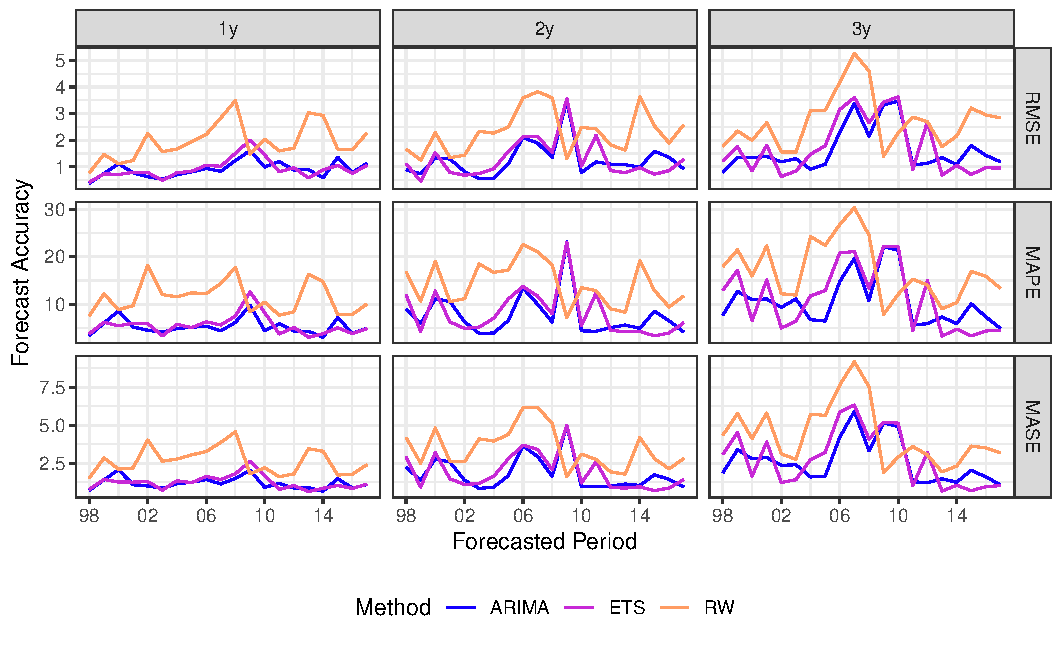
\includegraphics[width=\textwidth]{fig/fig_eval_methods_top}
	\caption{Accuracy of Forecasting Methods at the Top Level}
\end{figure}

\begin{figure}[H]
	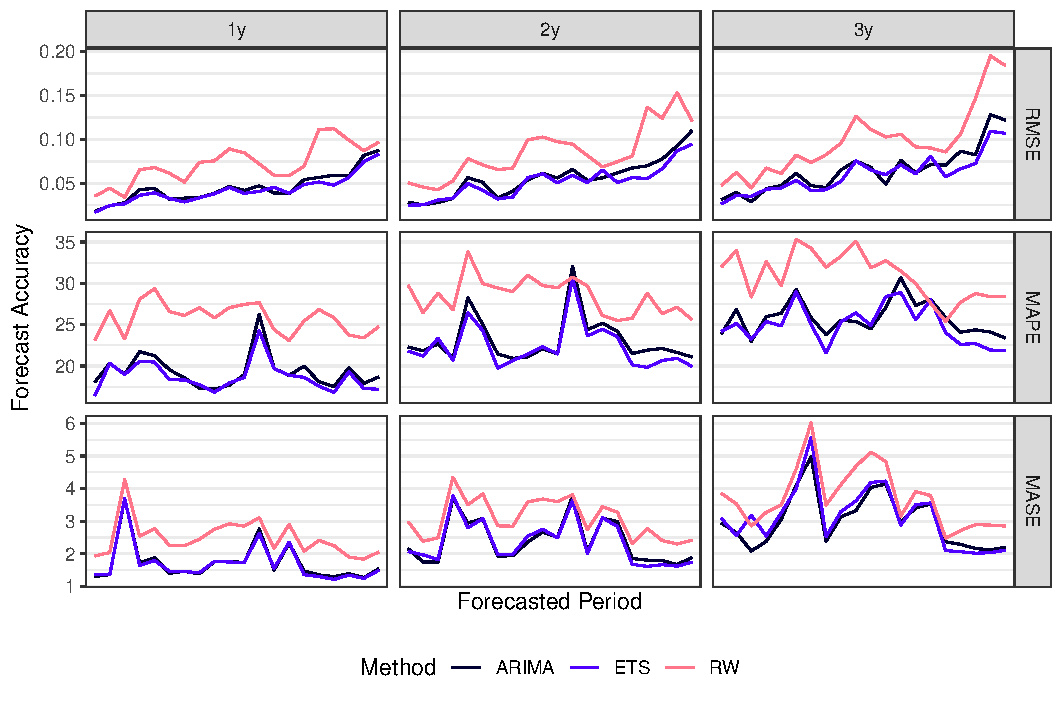
\includegraphics[width=\textwidth]{fig/fig_eval_methods_bottom}
	\caption{Accuracy of Forecasting Methods at the Bottom Level}
\end{figure}


\subsection{Data}
\label{sec:data}
The data is compiled by the Swiss Federal Customs Administration\footnote{\url{https://www.ezv.admin.ch/ezv/en/home/topics/swiss-foreign-trade-statistics.html}} and made available in a machine-friendly format on basis of a subscription.\\
% table with goods categories
\begin{small}
\begin{longtable}{p{2.5cm}p{11.5cm}}
\caption{Tariff Numbers and Descriptions of Goods}\\
\toprule
\normalsize{Tariff Number} & \normalsize{Description}\\
\midrule
\endfirsthead
\multicolumn{2}{@{}l}{\ldots continued}\\
\toprule
\normalsize{Tariff Number} & \normalsize{Description}\\  
\midrule
\endhead
\bottomrule
\multicolumn{2}{r@{}}{continued \ldots}\\
\endfoot
\bottomrule
\endlastfoot
	01	&	Forestry and agricultural products, fisheries	\\
\enskip	01.1	&	Food, beverages and tobacco	\\
\enskip	01.2	&	Feeding stuffs for animals	\\
\enskip	01.3	&	Live animals	\\
\enskip	01.4	&	Horticultural products	\\
\enskip	01.5	&	Forestry products (not firewood)	\\
\enskip	01.6	&	Products for commercial/industrial further processing such as oils, fats, starches, plants and vegetable parts, etc.	\\
\midrule
	02	&	Energy source	\\
\enskip	02.1	&	Solid combustibles	\\
\enskip	02.2	&	Petroleum and distillates	\\
\enskip	02.3	&	Gas	\\
\enskip	02.4	&	Electrical energy	\\
\midrule
	03	&	Textiles, clothing, shoes	\\
\enskip	03.1	&	Textiles	\\
\enskip	03.2	&	Articles of apparel and clothing	\\
\enskip	03.3	&	Shoes, parts and accessories	\\
\midrule
	04	&	Paper, articles of paper and and products of the printing industry	\\
\enskip	04.1	&	Basic materials for paper production, such as cellulose and cellulose fibre and paper and carton waste	\\
\enskip	04.2	&	Paper and carton in rolls, strips or sheets	\\
\enskip	04.3	&	Goods from paper or carton	\\
\enskip	04.4	&	Products of the printing industry	\\
\midrule
	05	&	Leather, rubber, plastics	\\
\enskip	05.1	&	Leather	\\
\enskip	05.2	&	Rubber	\\
\enskip	05.3	&	Plastics	\\
\midrule
	06	&	Products of the chemical and pharmaceutical industry	\\
\enskip	06.1	&	Chemical raw materials, basic materials and unformed plastics	\\
\enskip	06.2	&	Chemical end products, vitamins, diagnostic products, including active substances	\\
\midrule
	07	&	Stones and earth	\\
\enskip	07.1	&	Mineral raw materials and basic products	\\
\enskip	07.2	&	Goods from stone and cement	\\
\enskip	07.3	&	Ceramic wares	\\
\enskip	07.4	&	Glass	\\
\midrule
	08	&	Metals	\\
\enskip	08.1	&	Iron and steel	\\
\enskip	08.2	&	Non-ferrous metals	\\
\enskip	08.3	&	Metal goods	\\
\midrule
	09	&	Machines, appliances, electronics	\\
\enskip	09.1	&	Industrial machinery	\\
\enskip	09.2	&	Agricultural machines	\\
\enskip	09.3	&	Household appliances	\\
\enskip	09.4	&	Office machines	\\
\enskip	09.5	&	Electrical and electronic industry appliances and devices	\\
\enskip	09.6	&	Military equipment	\\
\midrule
	10	&	Vehicles	\\
\enskip	10.1	&	Road vehicles	\\
\enskip	10.2	&	Railed vehicles	\\
\enskip	10.3	&	Air- and spacecraft	\\
\enskip	10.4	&	Watercraft	\\
\midrule
	11	&	Precision instruments, clocks and watches and jewellery	\\
\enskip	11.1	&	Precision instruments and equipment	\\
\enskip	11.2	&	Watches	\\
\enskip	11.3	&	Jewellery and household goods made from precious metals	\\
\midrule
	12	&	Various goods such as music instruments, home furnishings, toys, sports equipment, etc.	\\
\enskip	12.1	&	Exposed film	\\
\enskip	12.2	&	Music instruments	\\
\enskip	12.3	&	Home furnishings	\\
\enskip	12.4	&	Toys and sports equipment	\\
\enskip	12.5	&	Stationery goods	\\
\enskip	12.6	&	Various goods such as umbrellas, neon signs, festive articles, brushes, lighters, pipes, etc.	\\
\midrule
	13	&	Precious metals, precious and semi-precious stones	\\
\enskip	13.1	&	Precious and semi-precious stones	\\
\enskip	13.2	&	Precious metals (including gold and silver bars from 1.1.2012)	\\
\midrule
	14	&	Works of art and antiques	\\
\enskip	14.1	&	Works of art	\\
\enskip	14.2	&	Antiques and collectors' items	\\
\end{longtable}
\end{small}

\clearpage

\begin{small}
	\begin{longtable}{p{7.5cm}cccc}
		\caption{Countries and Regional Aggregates}\\
		\toprule
Country	&	isoCode	&	regCode	&	valid from	&	valid to	\\
		\midrule
		\endfirsthead
		\multicolumn{4}{@{}l}{\ldots continued}\\
		\toprule
Country	&	isoCode	&	regCode	&	valid from	&	valid to	\\
		\midrule
		\endhead
		\bottomrule
		\multicolumn{4}{r@{}}{continued \ldots}\\
		\endfoot
		\bottomrule
		\endlastfoot
Switzerland	&	CH	&	EU	&	01/1988	&	-	\\
Germany	&	DE	&	EU	&	01/1988	&	-	\\
France	&	FR	&	EU	&	01/1988	&	-	\\
Italy	&	IT	&	EU	&	01/1988	&	-	\\
Netherlands	&	NL	&	EU	&	01/1988	&	-	\\
Belgium-Luxembourg	&	BE	&	EU	&	01/1988	&	12/1998	\\
Belgium	&	BE	&	EU	&	01/1999	&	-	\\
Luxembourg	&	LU	&	EU	&	01/1999	&	-	\\
Austria	&	AT	&	EU	&	01/1988	&	-	\\
United Kingdom	&	GB	&	EU	&	01/1988	&	-	\\
Denmark	&	DK	&	EU	&	01/1988	&	-	\\
Norway	&	NO	&	EU	&	01/1988	&	-	\\
Sweden	&	SE	&	EU	&	01/1988	&	-	\\
Portugal	&	PT	&	EU	&	01/1988	&	-	\\
Finland	&	FI	&	EU	&	01/1988	&	-	\\
Croatia, Republic of	&	HR	&	EU	&	02/1992	&	-	\\
Slovenia	&	SI	&	EU	&	02/1992	&	-	\\
Bosnia and Herzegovina	&	BA	&	EU	&	05/1992	&	-	\\
Macedonia	&	MK	&	EU	&	05/1992	&	-	\\
Montenegro	&	ME	&	EU	&	05/1992	&	12/1996	\\
Montenegro	&	ME	&	EU	&	01/2007	&	-	\\
Montenegro	&	XM	&	EU	&	01/2006	&	12/2006	\\
Serbia	&	SQ	&	EU	&	05/1992	&	12/1996	\\
Serbia	&	RS	&	EU	&	01/2007	&	-	\\
Serbia	&	XS	&	EU	&	01/2006	&	12/2006	\\
Federal Republic of Yugoslavia	&	YU	&	EU	&	01/1997	&	12/2003	\\
Serbia and Montenegro	&	CS	&	EU	&	01/2004	&	12/2005	\\
Kosovo	&	XK	&	EU	&	01/2006	&	-	\\
Iceland	&	IS	&	EU	&	01/1988	&	-	\\
Ireland	&	IE	&	EU	&	01/1988	&	-	\\
Spain	&	ES	&	EU	&	01/1988	&	-	\\
Greece	&	GR	&	EU	&	01/1988	&	-	\\
Turkey	&	TR	&	EU	&	01/1988	&	-	\\
GDR	&	DD	&	EU	&	01/1988	&	10/1990	\\
Poland	&	PL	&	EU	&	01/1988	&	-	\\
Czech Republic	&	CZ	&	EU	&	01/1993	&	-	\\
Czechoslovakia	&	CS	&	EU	&	01/1988	&	02/1992	\\
Slovakia	&	SK	&	EU	&	01/1993	&	-	\\
Hungary	&	HU	&	EU	&	01/1988	&	-	\\
Albania	&	AL	&	EU	&	01/1988	&	-	\\
Bulgaria, Republic of	&	BG	&	EU	&	01/1988	&	-	\\
Romania	&	RO	&	EU	&	01/1988	&	-	\\
USSR	&	SU	&	EU	&	01/1988	&	12/1991	\\
Yugoslavia	&	YU	&	EU	&	01/1988	&	04/1992	\\
Cyprus	&	CY	&	EU	&	01/1988	&	-	\\
Svalbard and Jan Mayen Island	&	SJ	&	EU	&	01/1999	&	-	\\
Malta	&	MT	&	EU	&	01/1988	&	-	\\
Gibraltar	&	GI	&	EU	&	01/1988	&	-	\\
Faeroe Islands	&	FO	&	EU	&	01/1988	&	-	\\
San Marino	&	SM	&	EU	&	01/1999	&	-	\\
Holy See	&	VA	&	EU	&	01/1999	&	-	\\
Andorra	&	AD	&	EU	&	01/1988	&	-	\\
Estonia	&	EE	&	EU	&	01/1992	&	-	\\
Latvia	&	LV	&	EU	&	01/1992	&	-	\\
Lithuania	&	LT	&	EU	&	01/1992	&	-	\\
Russian Federation	&	RU	&	CA	&	01/1992	&	-	\\
Armenia	&	AM	&	CA	&	01/1992	&	-	\\
Azerbaijan	&	AZ	&	CA	&	01/1992	&	-	\\
Belarus	&	BY	&	CA	&	01/1992	&	-	\\
Georgia	&	GE	&	CA	&	01/1992	&	-	\\
Kazakhstan	&	KZ	&	CA	&	01/1992	&	-	\\
Kyrgyz, Republic	&	KG	&	CA	&	01/1992	&	-	\\
Moldova, Republic of	&	MD	&	CA	&	01/1992	&	-	\\
Tajikistan	&	TJ	&	CA	&	01/1992	&	-	\\
Turkmenistan	&	TM	&	CA	&	01/1992	&	-	\\
Ukraine	&	UA	&	CA	&	01/1992	&	-	\\
Uzbekistan	&	UZ	&	CA	&	01/1992	&	-	\\
Egypt	&	EG	&	AF	&	01/1988	&	-	\\
Sudan	&	SD	&	AF	&	01/1988	&	-	\\
South Sudan, Republic of	&	SS	&	AF	&	09/2011	&	-	\\
Libya	&	LY	&	AF	&	01/1988	&	-	\\
Tunisia	&	TN	&	AF	&	01/1988	&	-	\\
Algeria	&	DZ	&	AF	&	01/1988	&	-	\\
Canary Islands	&	XA	&	AF	&	01/1988	&	-	\\
Morocco	&	MA	&	AF	&	01/1988	&	-	\\
Western Sahara	&	EH	&	AF	&	01/1999	&	-	\\
Ceuta and Melilla	&	XB	&	AF	&	01/1988	&	12/2010	\\
Equatorial Guinea	&	GQ	&	AF	&	01/1988	&	-	\\
Ceuta	&	XC	&	AF	&	01/2001	&	-	\\
Melilla	&	XL	&	AF	&	01/2001	&	-	\\
Togo	&	TG	&	AF	&	01/1988	&	-	\\
Senegal	&	SN	&	AF	&	01/1988	&	-	\\
Mali	&	ML	&	AF	&	01/1988	&	-	\\
Mauritania	&	MR	&	AF	&	01/1988	&	-	\\
Côte d'Ivoire	&	CI	&	AF	&	01/1988	&	-	\\
Burkina Faso	&	BF	&	AF	&	01/1988	&	-	\\
Benin	&	BJ	&	AF	&	01/1988	&	-	\\
Niger	&	NE	&	AF	&	01/1988	&	-	\\
Guinea	&	GN	&	AF	&	01/1988	&	-	\\
Gambia	&	GM	&	AF	&	01/1988	&	-	\\
Sierra Leone	&	SL	&	AF	&	01/1988	&	-	\\
Liberia	&	LR	&	AF	&	01/1988	&	-	\\
Ghana	&	GH	&	AF	&	01/1988	&	-	\\
Nigeria, Federal Republic of	&	NG	&	AF	&	01/1988	&	-	\\
Cameroon	&	CM	&	AF	&	01/1988	&	-	\\
Gabon	&	GA	&	AF	&	01/1988	&	-	\\
Congo, Republic of the	&	CG	&	AF	&	01/1988	&	-	\\
Central African Republic	&	CF	&	AF	&	01/1988	&	-	\\
Chad	&	TD	&	AF	&	01/1988	&	-	\\
Congo, Democratic Republic of the	&	CD	&	AF	&	06/1997	&	-	\\
Zaire	&	ZR	&	AF	&	01/1988	&	05/1997	\\
Angola	&	AO	&	AF	&	01/1988	&	-	\\
Guinea-Bissau	&	GW	&	AF	&	01/1988	&	-	\\
Botswana	&	BW	&	AF	&	01/1988	&	-	\\
Cabo Verde, Republic of	&	CV	&	AF	&	01/1988	&	-	\\
Lesotho	&	LS	&	AF	&	01/1988	&	-	\\
Sao Tomé and Principe	&	ST	&	AF	&	01/1988	&	-	\\
Namibia	&	NA	&	AF	&	01/1988	&	-	\\
South Africa	&	ZA	&	AF	&	01/1988	&	-	\\
Swaziland	&	SZ	&	AF	&	01/1988	&	-	\\
Zambia	&	ZM	&	AF	&	01/1988	&	-	\\
Zimbabwe	&	ZW	&	AF	&	01/1988	&	-	\\
Malawi	&	MW	&	AF	&	01/1988	&	-	\\
Mozambique	&	MZ	&	AF	&	01/1988	&	-	\\
Madagascar, Republic of	&	MG	&	AF	&	01/1988	&	-	\\
Réunion	&	RE	&	AF	&	01/1988	&	-	\\
St Helena, Ascen. and Tristan da Cunha	&	SH	&	AF	&	01/1988	&	-	\\
Comoros, Union of	&	KM	&	AF	&	01/1988	&	-	\\
Antarctica	&	AQ	&	AF	&	01/1988	&	-	\\
Mauritius	&	MU	&	AF	&	01/1988	&	-	\\
British Indian Ocean Territory	&	IO	&	AF	&	01/1988	&	-	\\
Tanzania, United Republic of	&	TZ	&	AF	&	01/1988	&	-	\\
Seychelles, Republic of	&	SC	&	AF	&	01/1988	&	-	\\
Rwanda	&	RW	&	AF	&	01/1988	&	-	\\
Bouvet Island	&	BV	&	AF	&	01/1999	&	-	\\
Burundi	&	BI	&	AF	&	01/1988	&	-	\\
Mayotte	&	YT	&	AF	&	01/1999	&	-	\\
Somalia, Federal Republic of	&	SO	&	AF	&	01/1988	&	-	\\
French Southern Territories	&	TF	&	AF	&	01/1999	&	-	\\
Djibouti	&	DJ	&	AF	&	01/1988	&	-	\\
Eritrea	&	ER	&	AF	&	01/1994	&	-	\\
Ethiopia, Fed. Democratic Republic of	&	ET	&	AF	&	01/1988	&	-	\\
Kenya	&	KE	&	AF	&	01/1988	&	-	\\
Uganda	&	UG	&	AF	&	01/1988	&	-	\\
Syrian Arab Republic	&	SY	&	AF	&	01/1988	&	-	\\
Lebanon	&	LB	&	AF	&	01/1988	&	-	\\
Israel	&	IL	&	AF	&	01/1988	&	-	\\
Palestine, the State of	&	PS	&	AF	&	01/1997	&	-	\\
Jordan	&	JO	&	AF	&	01/1988	&	-	\\
Saudi Arabia	&	SA	&	AF	&	01/1988	&	-	\\
Yemen (Nord)	&	YE	&	AF	&	01/1988	&	12/1990	\\
Yemen	&	YE	&	AF	&	01/1991	&	-	\\
Yemen (Sud)	&	YD	&	AF	&	01/1988	&	12/1990	\\
Qatar	&	QA	&	AF	&	01/1988	&	-	\\
Bahrain	&	BH	&	AF	&	01/1988	&	-	\\
United Arab Emirates	&	AE	&	AF	&	01/1988	&	-	\\
Oman	&	OM	&	AF	&	01/1988	&	-	\\
Kuwait	&	KW	&	AF	&	01/1988	&	-	\\
Iraq	&	IQ	&	AF	&	01/1988	&	-	\\
Iran, Islamic Republic of	&	IR	&	AF	&	01/1988	&	-	\\
Afghanistan	&	AF	&	SA	&	01/1988	&	-	\\
Pakistan	&	PK	&	SA	&	01/1988	&	-	\\
Bangladesh	&	BD	&	SA	&	01/1988	&	-	\\
India	&	IN	&	SA	&	01/1988	&	-	\\
Sri Lanka	&	LK	&	SA	&	01/1988	&	-	\\
Maldives	&	MV	&	SA	&	01/1988	&	-	\\
Nepal, Federal Democratic Rep.	&	NP	&	SA	&	01/1988	&	-	\\
Bhutan	&	BT	&	SA	&	01/1988	&	-	\\
Myanmar, Union of	&	MM	&	EA	&	01/1988	&	-	\\
Thailand	&	TH	&	EA	&	01/1988	&	-	\\
Malaysia	&	MY	&	EA	&	01/1988	&	-	\\
Brunei Darussalam	&	BN	&	EA	&	01/1988	&	-	\\
Singapore	&	SG	&	EA	&	01/1988	&	-	\\
Cambodia	&	KH	&	EA	&	01/1988	&	-	\\
Lao, People's Democratic Republic	&	LA	&	EA	&	01/1988	&	-	\\
Viet Nam, Socialist Republic of	&	VN	&	EA	&	01/1988	&	-	\\
Mongolia	&	MN	&	EA	&	01/1988	&	-	\\
China, People's Republic of	&	CN	&	EA	&	01/1988	&	-	\\
Hong Kong	&	HK	&	EA	&	01/1988	&	-	\\
Taiwan	&	TW	&	EA	&	01/1988	&	-	\\
Macau	&	MO	&	EA	&	01/1988	&	-	\\
Korea, People's Democratic Republic of	&	KP	&	EA	&	01/1988	&	-	\\
Korea, Republic of	&	KR	&	EA	&	01/1988	&	-	\\
Japan	&	JP	&	EA	&	01/1988	&	-	\\
Philippines	&	PH	&	EA	&	01/1988	&	-	\\
Indonesia	&	ID	&	EA	&	01/1988	&	-	\\
East Timor	&	TL	&	EA	&	01/2004	&	-	\\
East Timor	&	TP	&	EA	&	01/1999	&	12/2003	\\
Canada	&	CA	&	NA	&	01/1988	&	-	\\
St Pierre and Miquelon	&	PM	&	NA	&	01/1988	&	-	\\
United States	&	US	&	NA	&	01/1988	&	-	\\
Greenland	&	GL	&	NA	&	01/1988	&	-	\\
Mexico	&	MX	&	LA	&	01/1988	&	-	\\
Belize	&	BZ	&	LA	&	01/1988	&	-	\\
Guatemala	&	GT	&	LA	&	01/1988	&	-	\\
Honduras	&	HN	&	LA	&	01/1988	&	-	\\
El Salvador	&	SV	&	LA	&	01/1988	&	-	\\
Nicaragua	&	NI	&	LA	&	01/1988	&	-	\\
Costa Rica	&	CR	&	LA	&	01/1988	&	-	\\
Panama	&	PA	&	LA	&	01/1988	&	-	\\
Cayman Islands	&	KY	&	LA	&	01/1988	&	-	\\
Turks and Caicos Islands	&	TC	&	LA	&	01/1988	&	-	\\
Bahamas	&	BS	&	LA	&	01/1988	&	-	\\
Bermuda	&	BM	&	LA	&	01/1988	&	-	\\
Jamaica	&	JM	&	LA	&	01/1988	&	-	\\
Cuba	&	CU	&	LA	&	01/1988	&	-	\\
Haiti	&	HT	&	LA	&	01/1988	&	-	\\
Dominican Republic	&	DO	&	LA	&	01/1988	&	-	\\
American Virgin Islands	&	VI	&	LA	&	01/1988	&	-	\\
Puerto Rico	&	PR	&	LA	&	01/1988	&	12/2005	\\
Dominica	&	DM	&	LA	&	01/1988	&	-	\\
St Vincent and the Grenadines	&	VC	&	LA	&	01/1988	&	-	\\
St Lucia	&	LC	&	LA	&	01/1988	&	-	\\
Montserrat	&	MS	&	LA	&	01/1988	&	-	\\
Antigua and Barbuda	&	AG	&	LA	&	01/1988	&	-	\\
Barbados	&	BB	&	LA	&	01/1988	&	-	\\
Grenada	&	GD	&	LA	&	01/1988	&	-	\\
St Kitts and Nevis	&	KN	&	LA	&	01/1988	&	-	\\
Anguilla	&	AI	&	LA	&	01/1988	&	-	\\
Guadeloupe	&	GP	&	LA	&	01/1988	&	-	\\
British Virgin Islands	&	VG	&	LA	&	01/1999	&	-	\\
Martinique	&	MQ	&	LA	&	01/1988	&	-	\\
Trinidad and Tobago	&	TT	&	LA	&	01/1988	&	-	\\
Saint BarthÈlemy	&	BL	&	LA	&	01/2013	&	-	\\
Netherlands Antilles	&	AN	&	LA	&	01/1988	&	12/2012	\\
Aruba	&	AW	&	LA	&	01/1999	&	-	\\
Bonaire, Sint Eustatius and Saba	&	BQ	&	LA	&	01/2013	&	-	\\
Curacao	&	CW	&	LA	&	01/2013	&	-	\\
Sint Maarten (NL)	&	SX	&	LA	&	01/2013	&	-	\\
Colombia	&	CO	&	LA	&	01/1988	&	-	\\
Venezuela, the Bolivarian Republic of	&	VE	&	LA	&	01/1988	&	-	\\
Guyana	&	GY	&	LA	&	01/1988	&	-	\\
Suriname	&	SR	&	LA	&	01/1988	&	-	\\
French Guiana	&	GF	&	LA	&	01/1988	&	-	\\
Brazil	&	BR	&	LA	&	01/1988	&	-	\\
Paraguay	&	PY	&	LA	&	01/1988	&	-	\\
Uruguay	&	UY	&	LA	&	01/1988	&	-	\\
Argentina	&	AR	&	LA	&	01/1988	&	-	\\
Falkland Islands	&	FK	&	LA	&	01/1988	&	-	\\
South Georgia and South Sandwich Islands	&	GS	&	LA	&	01/1999	&	-	\\
Chile	&	CL	&	LA	&	01/1988	&	-	\\
Bolivia, the Plurinational State of	&	BO	&	LA	&	01/1988	&	-	\\
Peru	&	PE	&	LA	&	01/1988	&	-	\\
Ecuador	&	EC	&	LA	&	01/1988	&	-	\\
Australia	&	AU	&	AO	&	01/1988	&	-	\\
Papua New Guinea	&	PG	&	AO	&	01/1988	&	-	\\
Cocos (Keeling) Islands	&	CC	&	AO	&	01/1999	&	-	\\
Heard and McDonald Islands	&	HM	&	AO	&	01/1999	&	-	\\
Norfolk Island	&	NF	&	AO	&	01/1999	&	-	\\
Christmas Island	&	CX	&	AO	&	01/1999	&	-	\\
New Zealand	&	NZ	&	AO	&	01/1988	&	-	\\
Cook Islands	&	CK	&	AO	&	01/1998	&	-	\\
Samoa	&	WS	&	AO	&	01/1988	&	-	\\
Niue Island	&	NU	&	AO	&	01/1999	&	-	\\
Kiribati, the Republic of	&	KI	&	AO	&	01/1988	&	-	\\
Tokelau Islands	&	TK	&	AO	&	01/1999	&	-	\\
Tuvalu	&	TV	&	AO	&	01/1988	&	-	\\
Pitcairn Islands	&	PN	&	AO	&	01/1988	&	-	\\
Solomon Islands	&	SB	&	AO	&	01/1988	&	-	\\
French Polynesia	&	PF	&	AO	&	01/1988	&	-	\\
New Caledonia	&	NC	&	AO	&	01/1999	&	-	\\
Wallis and Futuna	&	WF	&	AO	&	01/1999	&	-	\\
American Oceania	&	PU	&	AO	&	01/1988	&	12/1996	\\
American Oceania	&	UM	&	AO	&	01/2006	&	-	\\
American Oceania	&	UM	&	AO	&	01/1997	&	12/2005	\\
Northern Mariana, Islands	&	MP	&	AO	&	01/1997	&	-	\\
Marshall Islands	&	MH	&	AO	&	01/1997	&	-	\\
Micronesia, Federated States of	&	FM	&	AO	&	01/1997	&	-	\\
Palau	&	PW	&	AO	&	01/1997	&	-	\\
Fiji, Republic of	&	FJ	&	AO	&	01/1988	&	-	\\
American Samoa	&	AS	&	AO	&	01/2006	&	-	\\
Guam	&	GU	&	AO	&	01/2006	&	-	\\
Vanuatu	&	VU	&	AO	&	01/1988	&	-	\\
Nauru	&	NR	&	AO	&	01/1988	&	-	\\
Tonga	&	TO	&	AO	&	01/1988	&	-	\\
Countries not specified	&	QX	&	EU	&	01/2002	&	-	\\
\end{longtable}
\end{small}

\subsection{Scaling Methods}
\label{subsec:scaling}
by equation (\ref{eq:scale}).
\begin{align}
	\label{eq:scale}
	|\lambda| &= \lambda_1 \lambda_2 \hdots \lambda_m
	= \prod_{s^- = 1}^{x} \lambda_{s^-}\ \eta^{-\frac{1}{x}}   \prod_{s^+ = x+1}^{m} \lambda_{s^+}\ \eta^{\frac{1}{m-x}} = 1
\end{align}
The $x$ local variance components $\lambda_{s^-}$ are scaled down by a factor $\eta^{\frac{1}{x}}$ and the remaining $(m-x)$ components $\lambda_{s^+}$ are correspondingly scaled up by a factor $\eta^{\frac{1}{m-x}}$. The generalized variance remains at unity irrespective of the scaling factor $\eta$ and the number of series to be scaled down $x$. 





\end{document}